\documentclass{pnastwo}
\usepackage{color}
\usepackage{graphicx}
\usepackage{amssymb,amsfonts,amsmath}
\usepackage{lineno}
\usepackage{multirow}
\usepackage{color}
	 \definecolor{darkred}{rgb}{0.75,0,0}
	 \definecolor{darkgreen}{rgb}{0,0.5,0}
	 \definecolor{darkblue}{rgb}{0,0,0.75}
\newcommand{\cha}[1]{\textcolor{darkblue}{#1}}
\newcommand{\arne}[1]{\textcolor{darkred}{#1}}


\usepackage[sort&compress]{}


\begin{document}

\title{Population dynamics of mutualisms}

 \author{Chaitanya S. Gokhale\affil{1}{New Zealand Institute for Advanced Study, Massey University, Auckland, New Zealand}}


\maketitle

\begin{article}

\begin{abstract}
Mutualistic relationships pose a conundrum for evolutionary theory.
Species that exploit other species would do better than sustaining a long drawn out mutually costly relationship. However we do see mutualistic relationships amongst even the most unlikely partners \ldots.
Eco-evolutionary dynamics \ldots
\end{abstract}


\keywords{mutualism | evolutionary game theory | multiple players
}

\section{Introduction}

In his book 'The History of Animals', Aristotle observes
{\em
`When the crocodile yawns, the trochilus flies into his mouth and cleans
his teeth. The trochilus gets his food thereby, and the crocodile
gets ease and comfort; it makes no attempt to injure its little friend,
but, when it wants it to go, it shakes its neck in warning, lest it
should accidentally bite the bird'} \cite{aristotle:350bc}.
In $1873$ the Belgian zoologist Pierre van Beneden termed this interaction as mutualism \cite{bronstein:book:2003}.
Mutualistic relationships, interspecific interactions that benefit both species, have been empirically studied for many years 
\cite{boucher:book:1985,hinton:PTENHS:1951,wilson:AmNat:1983,bronstein:QRB:1994,pierce:ARE:2002,kiers:Nature:2003,bshary:ASB:2004} and also a considerable body of theory has been put forth explaining the evolution and maintenance of such relationships \cite{poulin:JTB:1995,doebeli:PNAS:1998,noe:book:2001,johnstone:ECL:2002,bergstrom:PNAS:2003,hoeksema:AmNat:2003,akcay:PRSB:2007,bshary:Nature:2008}.
The example described by Aristotle and most other examples of mutualisms lend themselves to the idea of direct reciprocity \cite{trivers:QRB:1971} and have been thus extensively studied using evolutionary game theory.
The interactions in these models are usually dyadic.
A representative of each species is chosen and the outcome of the interactions between these representatives 
determines the evolutionary dynamics within each of the two species.
However, in many cases interactions between species cannot be reduced to such dyadic encounters \cite{stadler:book:2008}.

For example, in the interaction between ants and aphids or butterfly larvae \cite{pierce:BES:1987,hoelldobler:book:1990} many ants tend to these soft bodies creatures, providing them with shelter and protection from predation and parasites in exchange for honeydew, a rich source of food for the ants \cite{hill:OEC:1989,stadler:book:2008}.
This is not a one to one interaction between a larva and an ant, but rather a one to many interaction from the perspective of the larva.
Another well studied example is that of the plant-microbe mutualism where leguminous hosts prefer rhizobial symbionts that fix more nitrogen \cite{kiers:Nature:2003} or where plants provide more carbon resources to the fungal strains that are providing access to more nutrients \cite{kiers:Science:2011}.
However the interactions within the rhizobial symbionts community is usually ignored in the broader picture of the between species interactions however identifying and quantifying the intraspecific variation can be a daunting task \cite{behm:JE:2014}.
Similarly for the interactions between the cleaner fish and their hosts \cite{bshary:AB:2002,bshary:book:2003}. 
While the cohorts of cleaner fish together have been taken to determine the quality of a cleaning station, this can also drive variation of quality of cleaning within a cleaning station as per the interactions of individual cleaner fish amongst themselves.
\cha{Furthermore, since by definition mutualistic relationships are between species, it is natural to imagine that the observed relationship may be seasonal and the interactions as not a continuous feature of the evolutionary dynamics of a single species.
To assess the impact of this seasonality $\ldots$
In this manuscript we focus on this kind of -- possibly -- many to many interactions between two mutualistic species.}

In all, in this manuscript we look at the broader picture of mutualistic relationships and the ecology in which they are observed.
We study the the cumulative effect os the within species and between species interactions and the importance of these relationships, seasonality and population dynamics taken together.
To analyze how benefits are shared between the two mutualistic species, we make use of evolutionary game theory.
Since we consider the interaction of two species, we resort to bimatrix games
\cite{weibull:book:1995,hofbauer:JMB:1996,hofbauer:book:1998}.
While initially attempting to avoid the question of how mutualisms evolve in the first place, we see that when studying the complex dynamics which are possible due to the rest of the evolutionary as well as ecological factors, we indirectly explain the evolution of interspecific mutualism as a byproduct of a complex eco-evolutionary process.



\section{Model and Results}



Usually when interspecies relationships such as mutualism (or antagonist relationships as in predator-prey) are considered, the within species interactions are ignored for the sake of convenience. Including intraspecies interactions can however result in qualitatively different and rich dynamics.
In fact the coevolutionary dynamics between the two species is determined together by the inter as well as the intraspecific interactions.


\begin{figure}[h]
\begin{center}
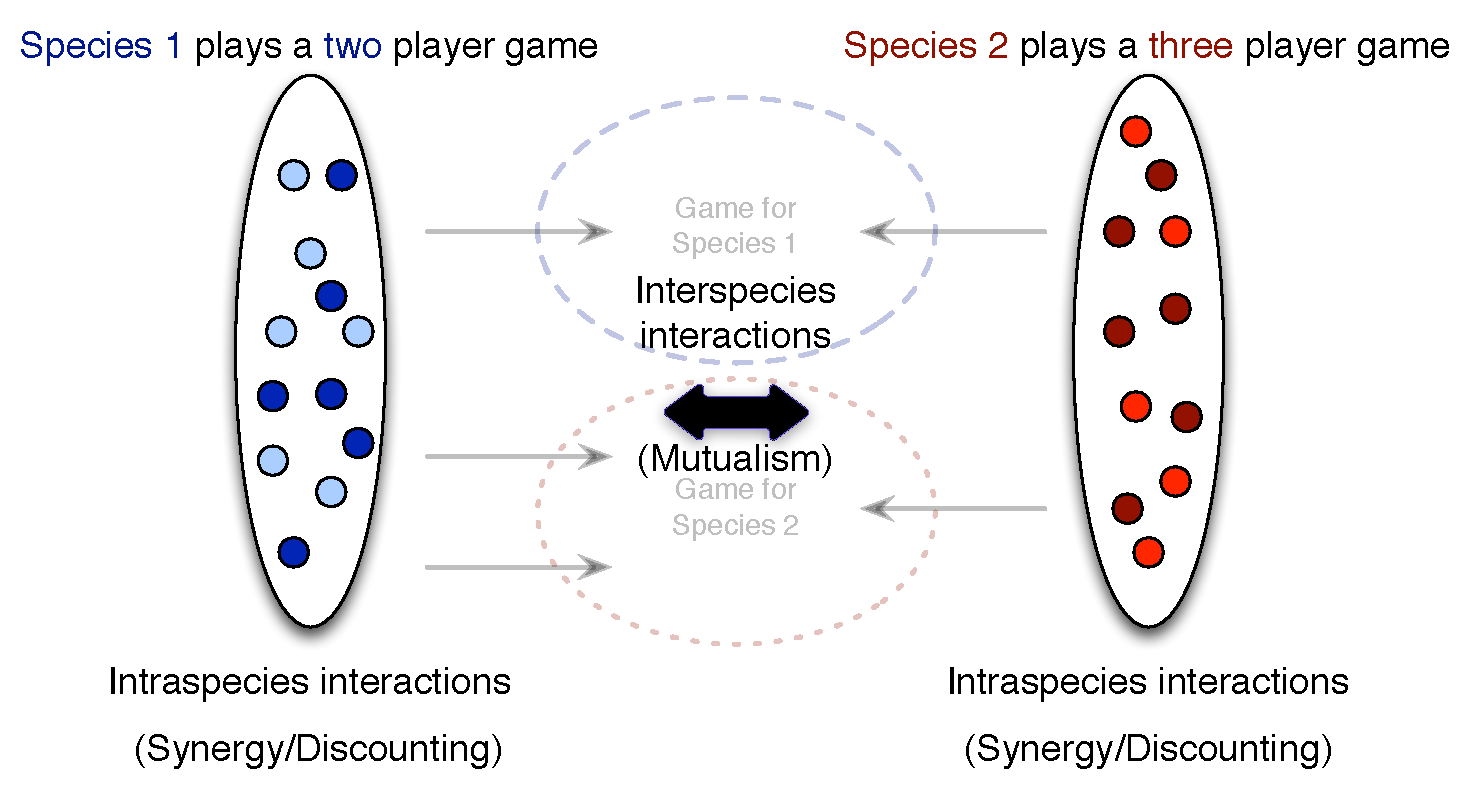
\includegraphics[width=\columnwidth]{../Figures/interintra.pdf}
\caption{
Explain figure
}
\end{center}
\end{figure}

\subsection{Interspecies dynamics}

Since we focus on mutualism the interspecies dynamics is given by the multiplayer version of the snowdrift game \cite{bergstrom:PNAS:2003,souza:JTB:2009,gokhale:PRSB:2012}.
Each species consists of two types of individuals Generous $G$ and Selfish $S$. 
The details of the game are included in the Supplementary Material (SI), but the gist is that if everyone is ``Generous" and contributing in the generation of mutual benefits then one can get away with being a bit selfish. However both species cannot be completely ``selfish" by definition of mutualism.
Hence the pressure is on a specie in making the partner ``Generous" while getting away itself by being ``Selfish".
The fitness of each of the types within a species thus depends on the composition of the other species.
For example if the frequency of the``Generous" types in Species $1$ ($G_1$) is $x$ and that in Species $2$ ($G_2$) is $y$ then fitness of $G_1$  is given by $f^{inter}_{G_1} (y)$ and that of $G_2$ as $f^{inter}_{G_2} (x)$

\subsection{Intraspecies dynamics}

We do not restrict ourselves to any particular interaction structure and thus can make use of the general multiplayer evolutionary games framework \cite{gokhale:PNAS:2010,gokhale:DGAA:2014}.
Moving from the interspecies dynamics, the two types already described are ``Generous" and ``Selfish".
Thus we already have each species containing two different types of individuals.
It is possible that a different categorisation exists within a species however for the sake of simplicity we study the dynamics between ``Generous" and ``Selfish" types within a species.
However the individuals which are ``Generous" for the interspecies interaction may/may not be more giving or in a sense ``Cooperators" for intraspecies dynamics.
Thus we need a flexible cost-benefit framework to model the intra species dynamics which can be easily tuned to the particular situation.
The cost benefit framework described in \cite{eshel:AmNat:1988,hauert:JTB:2006a}
 allows us to transition between four classic scenarios of evolutionary dynamics \cite{nowak:Science:2004}.

\cha{Describe the four outcomes}

For the intra species interactions the fitness of a $G_1$ is then given by $f^{intra}_{G_1} (x)$ and that of $G_2$ is given by $f^{intra}_{G_2} (y)$ and similarly for the ``Selfish" types.

\subsection{Combined dynamics}

Putting together intra and interspecific dynamics provides a complete picture of the possible interactions occurring. While we are interested in mutualism at the level of the interspecies interactions there are four possible interactions within each species \cite{nowak:Science:2004,hauert:JTB:2006a}. Since the within species interactions for the two different species do not need to be the same, there are in all sixteen different possible combinations.
Assuming additivity in the fitnesses of inter and intraspecies fitnesses, the combined fitness of each of the two types in the two species are given by,

%
\begin{align}
	f_{G_1} (x,y) &= p f^{inter}_{G_1} (y) + (1-p) f^{intra}_{G_1} (x) \\
	f_{S_1} (x,y) &= p f^{inter}_{S_1} (y) + (1-p) f^{intra}_{S_1} (x) \\
	f_{G_2} (x,y) &= p f^{inter}_{G_2} (x) + (1-p) f^{intra}_{G_2} (y) \\
	f_{S_2} (x,y) &= p f^{inter}_{S_2} (x) + (1-p) f^{intra}_{S_2} (y)
\end{align}
%
The parameter $p$ tunes the impact of each of the interactions on the actual fitness that eventually drives the evolutionary dynamics.
For $p=1$ we recover the well studied case of the Red King dynamics \cite{gokhale:PRSB:2012} while for $p=0$ the dynamics of the two species are essentially decoupled and can be individually studied by the synergy/discounting framework of nonlinear social dilemmas \cite{hauert:JTB:2006a}.
Of interest in the continuum and the intermediate values of $p$.
However that would mean we need to track the qualitative dynamics of sixteen possible intraspecies dynamics as $p$ changes gradually from close to $0$ to close to $1$ (SIix). 

This approach provides us with a powerful method to incorporate a lot of realistic concepts in the analysis.
For example the number of players involved in a game, which has been shown to be a crucial factor in determining the evolutionary dynamics could be different for each interactions, inter and intra species interactions for Species $1$ ($d^{inter}_1$,$d^{intra}_1$) and similarly for Species 2 ($d^{inter}_2$,$d^{intra}_2$). 
The interspecies interactions are proxied by the multiplayer Snowdrift game which can incorporate threshold effects.
For example a certain number of ``Generous" cleaner fish may be required to clean the host or a certain number of ``Generous" ants required to protect larva from predators.
We can have $M_1$ and $M_2$ as the thresholds in the two species.
Since the interaction matrices for the inter and intra species dynamics are completely different there doesn't need to be any relationship between the costs and benefits of the four games (Two snowdrift games from the perspective of each species and the intragames within each species).

 

\subsection{Population dynamics}
%Consider two species ($1/2$) occupying different niches in an ecosystem.
%Thus we assume them to have independent carrying capacities. Each species has a normalized carrying capacity of $1$. Each species has two types the \textit{``Generous"} ones ($G_{1/2}$) who invest in a mutualistic relationship with the other species and \textit{``Selfish"} ones ($S_{1/2}$) who invest much less than their counterparts. The densities of the two types are denoted by $x_{1/2}$ and $y_{1/2}$ respectively which can sum up to the carrying capacity or not thus resulting in possible empty spaces in the niche $z_{1,2}$. Thus in all we have $x_{1/2} + y_{1/2} + z_{1/2} = 1$.
%Thus how the population densities change over time $x_{1/2} + y(1/2)$ can give us a picture of the population dynamics.
%\subsection{Evolutionary dynamics}
%The two species are assumed to be engaged in a mutualistic relationship. This can be aptly described by a snowdrift game \cite{souza:JTB:2009}. In a general form, a number of individuals from one species interacts with a number of individuals from the other species (excluding intra species interactions) \cite{gokhale:PRSB:2012}. 
%The densities of the two types of individuals in each species \textit{``Generous"} and \textit{``Selfish"} can be interpreted as probabilities of picking the two types. Thus the evolution of the fraction of one of the types, say \textit{``Generous"} over time provides us with the relevant evolutionary dynamics. The fraction of \textit{``Generous"} players is given by $f_{1/2} = x_{1/2} / (1- z_{1/2} )$.



\section{Discussion}



\begin{acknowledgments}
Thanks for all the fish
\end{acknowledgments}




\bibliographystyle{pnas}
\bibliography{\string~/Bibtex/et.bib}


\end{article}
\end{document}